\documentclass[11pt,a4paper]{article}

%biblioteci
% \usepackage{times} % times new roman
\usepackage{csquotes} % pt warning
\usepackage{lipsum}
\usepackage{indentfirst} % pentru ca si primul paragraf sa aiba alineat
\usepackage{graphicx}  % pentru inserare imagini
\usepackage{float} % pt asezare imagini in pagina
\usepackage{hyperref} % pt cuprins cu linkuri catre sectiuni
\usepackage{minted} % pt cod

\usepackage{biblatex}
\usepackage{url}

% format document(margin)
\usepackage[top=2.5cm, bottom=2.5cm, left=2.5cm, right=2.5cm]{geometry}
\linespread{1.06} % spatiu intre cuvinte
\setlength{\parskip}{8pt plus2pt minus2pt} % spatiu intre paragrafe

% widow and orphan lines
\widowpenalty 10000
\clubpenalty 10000

\newcommand{\eat}[1]{}
\newcommand{\HRule}{\rule{\linewidth}{0.5mm}}

%puncte si dupa fiecare sectiune in cuprins
\usepackage{tocloft}
\renewcommand{\cftsecleader}{\cftdotfill{\cftdotsep}}

% pentru bibliografie
\usepackage{biblatex} % Imports biblatex package

% afiseaza mai frumos listele
\usepackage{enumitem} % ceva control asupra listelor/ enumerarilor
\setlist{nolistsep,noitemsep}

\setlength{\parskip}{2pt}  % spatiu intre paragrafe

% Fix for csquotes package
\DeclareQuoteStyle{nil}
{\textquotedblleft}
{\textquotedblright}
{\textquoteleft}
{\textquoteright}

% Fix for minted package
\usepackage{minted}
\usemintedstyle{default}

% Fix for biblatex package
\usepackage{biblatex}
\addbibresource{bibliography.bib} % Replace 'bibliography.bib' with the actual name of your bibliography file


\begin{document}

\begin{titlepage}
    \begin{center}

        % Title
        \HRule \\[0.4cm]
        { \LARGE
        \textbf{ChovL Documentation}\\[0.4cm]
        \emph{Formal languages and translators}\\[0.4cm]
        }
        \HRule \\[1.5cm]

        % Author
        { \large
        Author: Catalin Termure \\[0.1cm]
        Group: 30236\\[0.1cm]
        }

        \vfill
        \textsc{\large Facultatea de Automatica\\si Calculatoare}\\[0.4cm]

        % Bottom
        {\large 27 May 2024}

    \end{center}
\end{titlepage}
\tableofcontents % afiseaza cuprinsul
\section{Introduction}
ChovL is a simple compiled programming language, designed to be low-level, but still easy to use. It is a statically typed language, with a syntax similar to Rust.

\section{Technical Overview}
\subsection{Project structure}
Like most programming languages, ChovL is split into a lexer, parser, and code generator. The lexer and parser are implemented using Flex and Bison, respectively. The code generator is implemented in C++ and uses LLVM libraries to generate LLVM IR code. The LLVM IR code is then compiled to machine code by the LLVM compiler. This means that ChovL can run on any platform that LLVM supports and can use libraries written in C with the help of the LLVM linker.

ChovL also has a VSCode plugin that provides basic syntax highlighting:

\begin{center}
  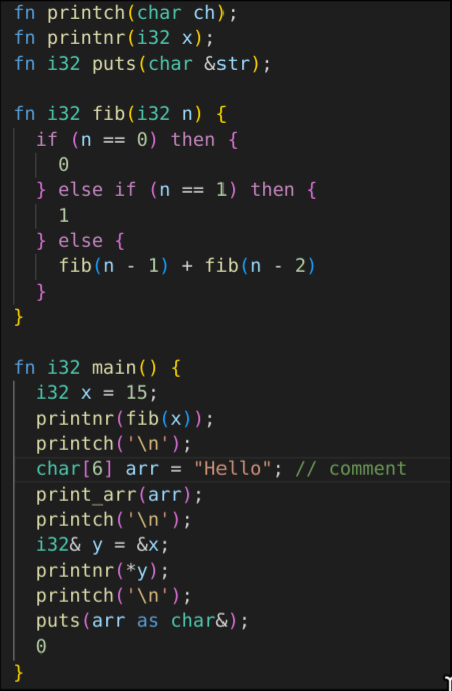
\includegraphics[width=0.4\textwidth]{images/vscode.png}
\end{center}

\subsection{Development Environment}
The project is developed in C++ and uses CMake as the build system. The project depends on:
\begin{itemize}
  \item A C++20 compiler(this was developed with GCC 13.2.0)
  \item \texttt{cmake} for building the project
  \item \texttt{flex} for the lexer
  \item \texttt{libbison-dev} for the parser
  \item \texttt{llvm-18} for the code generator
\end{itemize}

The best way to build the project is using the VSCode CMake extension.
If you want to build the project manually, you can use the following commands:
\begin{minted}{bash}
mkdir build
cd build
cmake ..
ninja # or make
\end{minted}

There is also an example project in the \texttt{example} directory for testing the language. You can build it by using the \texttt{make} command in the \texttt{example} directory.

\section{Syntax}
\subsection{Comments}
Comments in ChovL are only single-line comments and are started with the \texttt{//} characters, like in C/C++.

\subsection{Variables}

\subsubsection{Types}

ChovL has the following primitive types:
\begin{itemize}
  \item \texttt{i32} - 32-bit signed integer
  \item \texttt{f32} - 32-bit floating-point number
  \item \texttt{char} - character value
\end{itemize}

You may also have arrays of primitive types and pointers to a primitive type.

ChovL is strongly typed, so you cannot assign a value of one type to a variable of another type. You can, however, cast a value to another type using the \texttt{as} operator.
\begin{minted}{rust}
  i32 a = 5;
  f32 b = a as f32;
\end{minted}

\subsubsection{Declaration}

Variables are declared similar to C/C++, with the exception of array declarations and pointers. The syntax for variable declarations is as follows:
\begin{minted}{rust}
  i32 a = 5;
  f32 b = 3.14;
  char c = 'a';
  char[6] d = "Hello"; // Notice the 6 = 5 + 1 for the null terminator
  i32& e = &a; // e is a pointer to a
\end{minted}

\subsection{Statements and Expressions}
\subsubsection{Description}
Statements and expressions in ChovL are similar to C/C++. Statements are terminated with a semicolon, and expressions are evaluated and return a value. The following are examples of statements and expressions:
\begin{minted}{rust}
  {
    i32 a = 5; // this is a statement
    i32 b = 6; // this is a statement
    a + b // this is an expression
  }
\end{minted}

\subsubsection{Operations}
ChovL supports the following operations:
\begin{itemize}
  \item Arithmetic operations: \texttt{+}, \texttt{-}, \texttt{*}, \texttt{/}, \texttt{\%}
  \item Comparison operations: \texttt{==}, \texttt{!=}, \texttt{<}, \texttt{>}, \texttt{<=}, \texttt{>=}
  \item Logical operations: \texttt{\&\&}, \texttt{||}
  \item Assignment: \texttt{=}
  \item Cast operations: \texttt{as}
\end{itemize}

ChovL also supports a special assignment, called multi-assignment, which allows you to assign multiple values to multiple variables at once. The syntax for multi-assignment is as follows:
\begin{minted}{rust}
  i32 x = 5;
  i32 y = 7;
  {x, y} = {10, 25};
\end{minted}

\subsection{Blocks}
Blocks are declared using curly braces, similar to C/C++:
\begin{minted}{rust}
  {
    i32 a = 5;
    i32 b = 6;
    a + b;
  }
\end{minted}

Blocks are special in ChovL because they can be expressions if they end with an expression, not a statement. This means that the last statement in a block is the return value of the block.
\begin{minted}{rust}
  i32 a = {
    i32 b = 5;
    i32 c = 6;
    b + c
  };
\end{minted}

But blocks are not functions, so the statements in a block preceding the last expression are evaluated before the expression in which they appear. Each block is evaluated in the order of evaluation of the expression they replace.

Blocks also have a scope, so variables declared in a block are only accessible within that block.

\subsection{Control Flow}
ChovL supports function calls and if statements for control flow. The syntax for if statements is as follows:
\begin{minted}{rust}
  if (a == 5) then {
    a = 6;
  } else {
    a = 7;
  }
\end{minted}

There are also if expressions, which are similar to if statements, but they return a value:
\begin{minted}{rust}
  i32 a = if (b == 5) then {
    6
  } else {
    7
  };
  // or the shorter version
  i32 a = if (b == 5) then 6 else 7;
\end{minted}

\subsection{Functions}
Functions are declared using the \texttt{fn} keyword, followed by the function name, arguments, and return type. The syntax for function declarations is as follows:
\begin{minted}{rust}
  fn add(i32 a, i32 b) -> i32 {
    a + b
  }
\end{minted}

There is also a C-style declaration for functions, where the return type is specified before the function name:
\begin{minted}{rust}
  fn i32 add(i32 a, i32 b) {
    a + b
  }
\end{minted}

Functions may also be declared with an assignment operator:
\begin{minted}{rust}
  fn i32 add(i32 a, i32 b) = a + b;
\end{minted}

Functions may also be declared without being defined, like in C/C++. This lets you declare a function in one file and define it in another file, or pull in a function from a library:
\begin{minted}{rust}
  fn i32 add(i32 a, i32 b);
  fn i32 puts(char& string); // puts is a function from the C standard library
\end{minted}

\section{Implementation Details}
\subsection{Overview}
The ChovL compiler is split into three main parts: the lexer, the parser, and the code generator. The lexer reads the input file and tokenizes it, the parser reads the tokens and generates an abstract syntax tree, and the code generator reads the abstract syntax tree and generates LLVM IR code.

\subsection{Lexer}
The lexer is implemented using Flex. It reads the input file and tries to tokenize it. Every token has a type and only some tokens have a value. If we encounter anything that is not a recognized token, the program immediately exits with an error message. This means that everything we pass to the lexer will be a token.

\subsection{Parser}

The parser is implemented using Bison. It reads the tokens generated by the lexer and generates an abstract syntax tree that mostly mirrors the grammar of the language, with all non-terminals corresponding to an instance of a base abstract class called \texttt{ASTNode}. Some non-terminals may be subclasses of \texttt{ASTNode}, like \texttt{AssignableNode} or \texttt{ASTAggregateNode}. One notable exception is function arguments, which don't need any code generation, but still have to be parsed separately.

\subsection{Code generator}
Generating code for an AST is done in a bottom-up manner, by recursively generating code for the children of a node before generating code for the node itself. This allows us to generate code for complex expressions, like function calls or if statements quite easily.

There are some issues that arise with AST nodes that have multiple possible generation paths. For example, casting an array to a pointer is not actually a cast instruction, it's a pointer to the first element of the array. For all other cases, we care about the value, not the memory address of the operand of the cast. This means that we have to generate different code for this type of cast.

The code generator was inspired by the LLVM IR generated by clang, by looking at the equivalent C code and the generated LLVM IR. This allowed me to generate code that is similar in efficiency to the code generated by clang.

\subsubsection{Scoping}
Scoping is a common problem in programming languages. The way I solved scoping in ChovL is by using a stack of scopes. Each scope is a map of variable names to their values. When a new block is entered, a new scope is pushed onto the stack. When a block is exited, the scope is popped off the stack. I use a dynamic array to store the scopes, since we may need to access variables outside the innermost scope.

Looking up a symbol is done by iterating over the scopes from the innermost scope to the outermost scope, and returning the first scope that contains the symbol. This also allows us to shadow variables in inner scopes.

\section{Testing}
Testing is done using CTest, which is a part of CMake. The tests are located in the \texttt{tests} directory and are run using the \texttt{ctest} command. We use two types of tests: diff tests and validation tests. Diff tests compare the output of the compiled program with the expected output, and validation tests check if the compiled program is valid.

There are currently 24 test cases, each testing a different feature of the language and each having both a diff test and a validation test.

An example of a test is as follows:
\begin{center}
  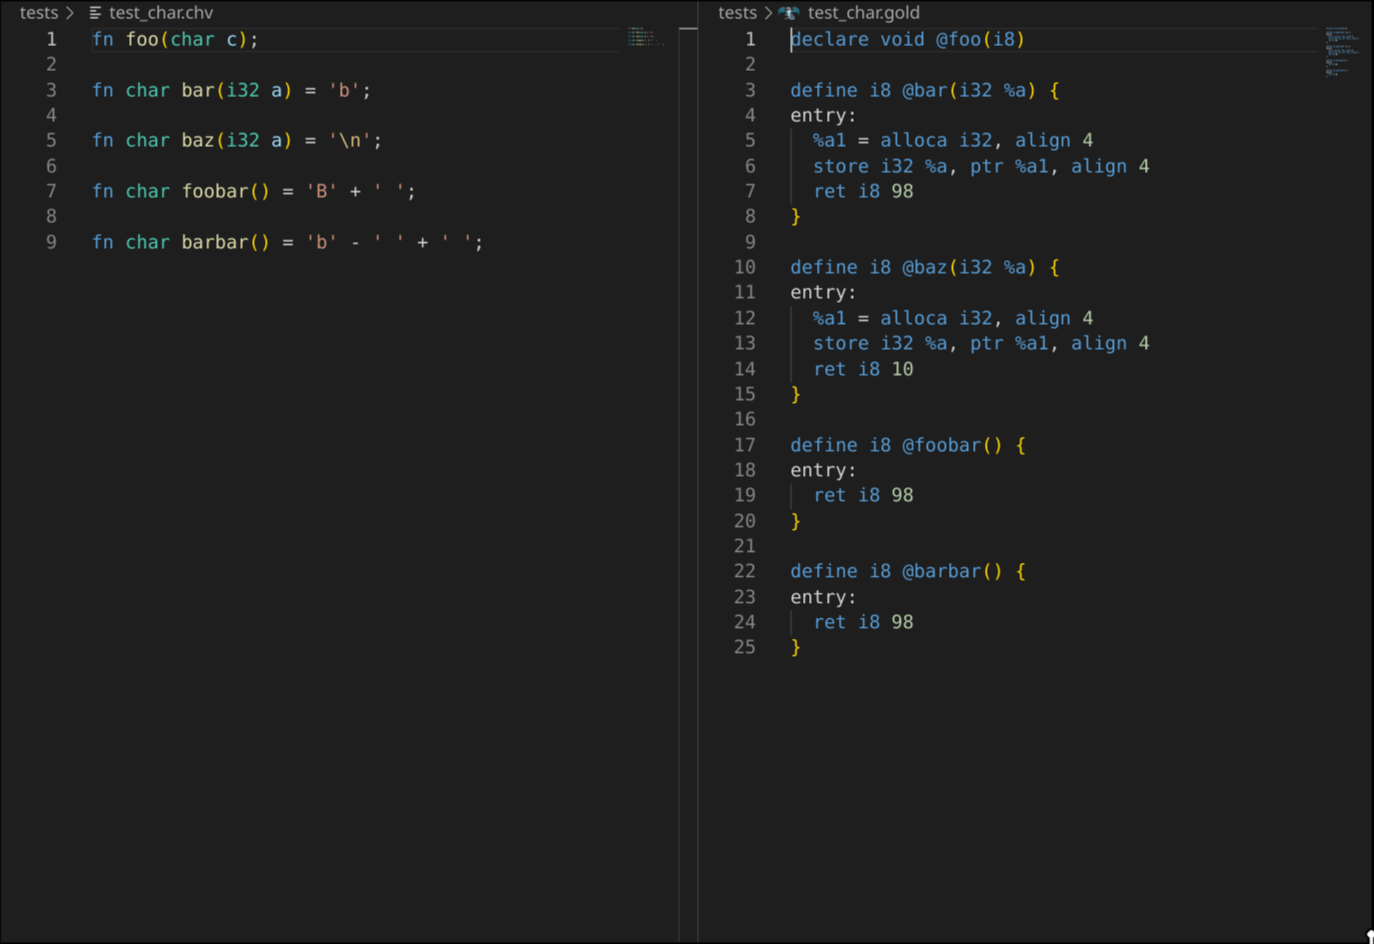
\includegraphics[width=1\textwidth]{images/test_example.png}
\end{center}

\section{Retrospective}
\subsection{Strong points}
\begin{itemize}
  \item The language is simple and easy to use
  \item The language is low-level and can be used for systems programming
  \item The language is statically typed, which helps catch errors at compile time
  \item The language is compiled to LLVM IR, which allows it to run on any platform that LLVM supports
  \item The language can use the LLVM optimizer to optimize the generated code
  \item The language has a VSCode plugin that provides basic syntax highlighting
\end{itemize}

\subsection{Weak points}
\begin{itemize}
  \item The language is not as feature-rich as other languages like C/C++ or Rust
  \item There are very few data types in the language
  \item Debugging is hard because the language does not have a debugger, leaving you to rely on print statements or assembly-level debugging
  \item The language does not have a standard library, so you have to write your own functions for common tasks
  \item There are no imports or modules, so you have to forward declare functions if you want to pull them from another file or library
\end{itemize}

\subsection{Future Work}
\begin{itemize}
  \item Add more data types to the language
  \item Add a standard library to the language
  \item Add a debugger to the language
  \item Add imports or modules to the language
  \item Add more control flow statements to the language like loops
  \item Add more operations to the language
  \item Add dynamic memory allocation to the language
\end{itemize}

\section{Conclusion}
ChovL is a simple compiled programming language, designed to be low-level, but still easy to use. It is a statically typed language, with a syntax similar to Rust. The language is simple and easy to use, but it lacks some features that other languages have. The language is compiled to LLVM IR, which allows it to run on any platform that LLVM supports. The language has a VSCode plugin that provides basic syntax highlighting.

This language isn't quite ready to be used for small projects, but it's not impossible to use for small tasks, which was the main goal of the project.

I learned a lot about compilers and programming languages while working on this project. The generated LLVM IR was inspired from the LLVM IR generated by clang, so I learned a lot about how clang generates LLVM IR from C++ code. I've had to think about how to solve some common problems in implementing a programming language, like scoping, error messages, AST nodes that have multiple possible generation paths. % documentatia propriu-zisa

\end{document}
